\documentclass{article}
\usepackage[utf8]{inputenc}
\usepackage{geometry}
 \geometry{
 a4paper,
 total={170mm,257mm},
 left=20mm,
 top=20mm,
 }


\usepackage{algorithm}
\usepackage{algpseudocode}
\usepackage{amsmath}
\usepackage{amsfonts}
\usepackage{amssymb}
\usepackage[spanish]{babel}
\usepackage{hyperref} 
\usepackage{graphicx}
\usepackage{bera}
\usepackage{listings}
\usepackage{xcolor}

\colorlet{punct}{red!60!black}
\definecolor{background}{HTML}{EEEEEE}
\definecolor{delim}{RGB}{20,105,176}
\colorlet{numb}{magenta!60!black}



\lstdefinelanguage{json}{
    basicstyle=\normalfont\ttfamily,
    numbers=left,
    numberstyle=\scriptsize,
    stepnumber=1,
    numbersep=8pt,
    showstringspaces=false,
    breaklines=true,
    frame=lines,
    backgroundcolor=\color{background},
    literate=
     *{0}{{{\color{numb}0}}}{1}
      {1}{{{\color{numb}1}}}{1}
      {2}{{{\color{numb}2}}}{1}
      {3}{{{\color{numb}3}}}{1}
      {4}{{{\color{numb}4}}}{1}
      {5}{{{\color{numb}5}}}{1}
      {6}{{{\color{numb}6}}}{1}
      {7}{{{\color{numb}7}}}{1}
      {8}{{{\color{numb}8}}}{1}
      {9}{{{\color{numb}9}}}{1}
      {:}{{{\color{punct}{:}}}}{1}
      {,}{{{\color{punct}{,}}}}{1}
      {\{}{{{\color{delim}{\{}}}}{1}
      {\}}{{{\color{delim}{\}}}}}{1}
      {[}{{{\color{delim}{[}}}}{1}
      {]}{{{\color{delim}{]}}}}{1},
}




\makeatletter
\renewcommand{\ALG@name}{Algoritmo}
\renewcommand{\listalgorithmname}{Lista de \ALG@name s}
\makeatother

\title{Proyecto 1 Modelado y Programacion}
\author{Ricardo Emiliano Apodaca Cardiel}
\date{}


\begin{document}

    \maketitle
    \tableofcontents


    \newpage

    \section{El problema}

    El problema requiere que se muestre el clima de las ciudades que deseen los sobrecargos y pilotos de manera facil y sencilla.


    \section{Entendiendo el problema}
    \label{sec:EntProb}
    Para empezar lo que se desea obtener el el clima ciudades, mas concretamente de aeropuetos ya que
la aplicación va a dirigida hacia pilotos y sobrecargos, para esto la aplicación tendra una interfaz gráfica
para la facilidad de uso al usuario, que en este caso son pilotos y sobrecargos.

Notemso que no es necesario mostrar la ciudad de origen ya que los mismos, pilotos y sobrecargos, ya que se encuentran ahi, o si
desean saber el clima exacto pueden solicitarlo como se mostrara en breves y como los usuario estan dentro del mundo de la aviacion
es de esperar que conozcan tanto los codigos IATA como ICAO, por lo que solicitaremos estos datos para saber de donde obtener el clima
del lugar deseado.

Si es posible encontrar el clima del lugar, esto se discutira mas adelante en sección \ref{sec:Procesos}, se le mostara al usuario, al igual que si hubo problemas.

Por lo que de entrada se requerira el codigo IATA o ICAO del aueropuerto que se desee saber el clima, y de salida se le mostrara este al usuario.


    \section{Arsenal}
    \label{sec:Arsenal}
    \subsection{Lenguaje y Herramientas}
\label{subsec:LengHerr}

Para este proyecto se decidio que se utilizara \href{https://www.swift.org}{Swift} para la crecion de este. Ya que nos
permitira crear la aplicación para dispotivos iOS, macOs, y iPadOS, para facilitar el uso de la aplicación. Aparte de esto se
utilizara el framework de \href{https://developer.apple.com/documentation/swiftui/}{SwiftUI} proporcionado por Apple para crear la
interfaz grafica, debido a todos los elementos que nos propociona y la facilidad de uso. Y sera desarollada en en la IDE, Xcode, debido a todas las herramientas que propociona para el desarrollo para
dentro del enterno de Apple.


\subsection{API}
\label{subsec:API}
Tambien para la API se decidió por \href{https://www.checkwxapi.com}{CheckWXAPI} ya que usa el codigo ICAO como base para las peticiones,
y nos da todo lo que requerimos como el clima y mas datos, que podrian resultar ser utiles. Una API sera necesaria, la expliación en la
sección \ref{sec:Requisitos}.

    \newpage

    \section{Requistos}
    \label{sec:Requisitos}
    La aplicación requerira varias condiciones para su funcinamiento optimo, primero descutiremso los requisitos funcionales, despues
los no-funcionales, y por ultimo rapidamente lo que se requerira de parte del usuario.

\subsection{Requisitos Funcionales}
\begin{itemize}
    \item Entregar el clima del aeropueto deseado. Como se vio en la sección \ref{sec:EntProb}.
    \item Solicitar al usuario el codigo ICAO o IATA del aeropueto del que se desee saber el clima.
    \item Hacer la llamada a la API, si es necesaria, mencionada en la sección \ref{sec:Arsenal} y procesar la informacion para presentarsela
    usuario.
    \item Tener un Cache para almacenar el clima de locaciones solicitadas recientemente para no hacer llamadas inecesarias a la API. Si
    la informacion tiene una antiguedad $t$, desecharla y solicitar una nueva a la API. 
    \item  Si no es posible obtener la informacion del clima, informale de esto al usuario.
    \item Debido a que la API solo acepta codigo ICAO, tranformar de IATA al codigo ICAO correspondiente.
    \item Presentarle la información del clima deseada al usuario en la interfaz gráfica.
\end{itemize}

\subsection{Requisitos No-Funcionales}
\begin{itemize}
    \item Eficiencia y resposibidad por parte de la interfaz gráfica.
    \item Tolerar que el usuario ingrese un codigo inexiste o incorrecto, y si es posible informarle de su error, como por ejemplo,
    caracteres extra, o falta, o si es posible si los codigos que esta proporcionando no existen.
    \item Interfaz sencilla y autoexplicativa.
    \item Seguridad al guarda la llave de la API del usuario.
    \item Un manual de usuario integrado en la aplicación.
\end{itemize}

\subsection{Requerimiento por Parte del Usuario}
\begin{itemize}
    \item Una coneccion a internet por parte del usuario para acceder a la API y obtener los climas, ya que son esto no es posible acceder a la API.
    \item Ingresar correctamente el aeropueto, ya que aunque podemos decirle al usuario el error, necesitamos saber concretamente a cual se refiere.
\end{itemize}

Con esto tenemos todo los requerimientos basicos por parte de la aplicación, aunque aun pueden ser modificados y sirguir nuevos conforme avance
el proyecto.
    \newpage


    \section{Procesos}
    \label{sec:Procesos}
    Ahora se mostraran los procesos y el funcionamiento interno de la aplicación, los metodos, funciones, estructuras y clases.

La manera en que funcioanra la aplicación, com ya se menciono sera con una interfaz gráfica para el usuario, la cual estara comunicandose
con el modelo de la aplicación. La disposicion en la figura \ref{fig:UIDiagrama} una idea de la disposicion de la interfaz gráfica.
\begin{figure}[ht]
    \label{fig:UIDiagrama}
    \caption{Disposicion de la aplicación}
    \centering
    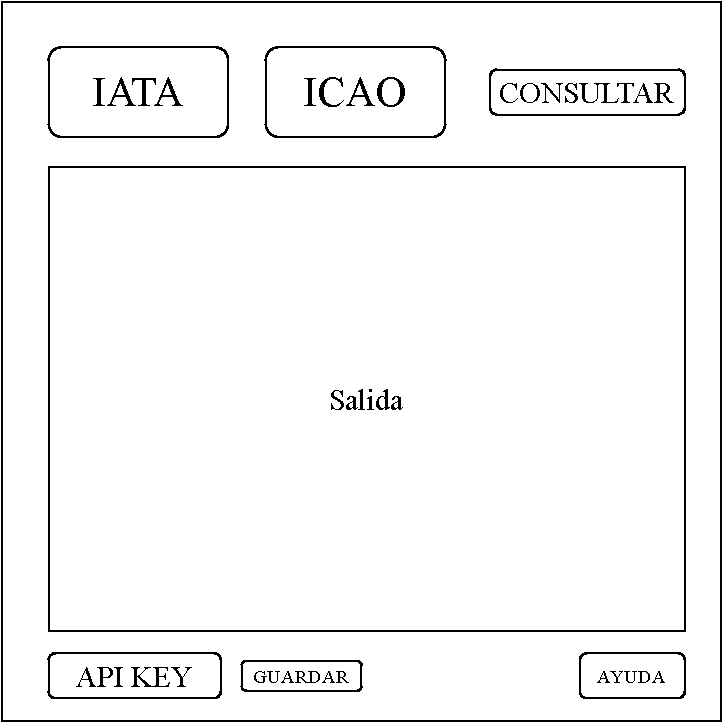
\includegraphics[width=\textwidth]{Figuras/UIDiagram.pdf}
\end{figure}

Las entradas serian los campos de AITA y IACO, mientras que tambien sera necesario que se proporcione una llave para la API, por lo
que seria otra entrada, ya que no es seguro incluir en el codigo, por lo que se requeria que el usuario proporcione su llave, tambien
se vera la posibilidad de guardar la llave en memoria para la comodidad del usuario.

Ahora pasando al modelo, veremos lo que lo va a conformar. Seguiremos el camino que seguiria los datos de entrada en el programa.

\subsection{Algoritmos}

Primero reciberemos la informacion recibida a travez de la interfaz, pero hay que tomar en cuanta que como tenemos 2 tipos de entrada, 
la IATA y la ICAO, por lo que se hara que la interfaz solo reciba 1 al mismo tiempo. Por otro lado recordemos que la API que se presento
en la sección \ref{subsec:API} de Arsenal, funciona con ICAO, no IATA, por lo que deberemos transformar el codigo IATA a ICAO.

\begin{algorithm}
    \caption{Tranforma de IATA a ICAO}\label{alg:IATA_TO_IACO}
    \begin{algorithmic}
        \Require Codigo IATA
        \State Primera concidencia de la base de datos del codigo IATA
        \Return Codigo ICAO de la coincidencia de la base de datos.
    \end{algorithmic}
\end{algorithm}

Despues de conseguir el codigo ICAO, ya sea directamente del usuario o por medio del algoritmo \ref{alg:IATA_TO_IACO},
seguira segura hacer la consulta del clima, para esto se tendra la cache como un diccionario con llaves de tipo \texttt{String},
las cuales seran el codigo ICAO, y valores  [\texttt{Información del Clima}] y \texttt{Date} para la cache. Pero para esto definamos primero como guardaremos la informacion. 
Sera en un arreglo,y las estructuras del arreglo sera de la siguiente manera:

\textbf{Información del Clima}
\begin{itemize}
    \label{strc:info}
    \item Codigo ICAO
    \item Codigo IATA
    \item Barometro
    \item Nubes
    \item Humedad
    \item Coordenadas
    \item Locación
    \item Nombre
    \item Temperatura
    \item Visibilidad
    \item Viento
    \item Tiempo de solicitud
\end{itemize}

Se incluira esto debido a que incluye la informacion basica asi como un poco de avanzada que puede llegar a ser de utilida a pilotos, aprte
que la respuesta de la API en METAR, que es un formato para ver el clima actual, se ve de esta manera.

\begin{lstlisting}[language=json,firstnumber=1]
    {
  "results": 1,
  "data": [
    {
      "barometer": {
        "hg": 30.02,
        "hpa": 1017.0,
        "kpa": 101.66,
        "mb": 1016.62
      },
      "clouds": [
        {
          "code": "CLR",
          "text": "Clear skies"
        }
      ],
      "dewpoint": {
        "celsius": 21,
        "fahrenheit": 70
      },
      "elevation": {
        "feet": 3,
        "meters": 1
      },
      "flight_category": "VFR",
      "humidity": {
        "percent": 79
      },
      "icao": "KPIE",
      "observed": "2021-04-30T23:53Z",
      "raw_text": "KPIE 302353Z AUTO 31009KT 10SM CLR 25/21 A3002 RMK AO2 SLP165 T02500206 10300 20250 55001",
      "station": {
        "geometry": {
          "coordinates": [
            -82.687401,
            27.9102
          ],
          "type": "Point"
        },
        "icao": "KPIE",
        "location": "St Petersburg-Clearwater, FL, USA",
        "name": "St Petersburg Clearwater International Airport",
        "type": "Airport"
      },
      "temperature": {
        "celsius": 25,
        "fahrenheit": 77
      },
      "visibility": {
        "meters": "16,000",
        "meters_float": 16000,
        "miles": "10",
        "miles_float": 10.0
      },
      "wind": {
        "degrees": 310,
        "speed_kph": 17,
        "speed_kts": 9,
        "speed_mph": 10,
        "speed_mps": 5
      }
    }
  ]
}
\end{lstlisting}

Ahora ya podemos pasar a ver como consultaremos el clima de un lugar. Este estara contenido en una estructura la cual sera la encargada
de manejar la informacion dependiendo de lo que se le vaya solicitando la que tenga el diccionario con todos los climas.
Tendra nadamas 2 atributos, ambos privados, los cuales seran el diccionario.
\texttt{InformacionClimas} prevamiente mencionado y la llave de la API.

\begin{algorithm}
    \caption{Algorimo para conseguir la informacion de clima de un lugar}\label{alg:prosClima}
    \begin{algorithmic}
        \Require Codigo ICAO(ICAO), Llave de API(API\_KEY)
        \State \texttt{solicitud\_actual} $\gets$ \texttt{InformacionClimas[ICAO]}
        \If{\texttt{solicitud\_actual} no existe o es muy vieja}
            \State $x \gets$ peticioAPI \Comment{PeticionAPI sera otra funcion dentro de la estructura}
            \If{La llamada fue exitosa}\\
                \State \texttt{solicitud\_actual} $\gets x$ 
            \Else\\
                \Return Llamada a la API fallida
            \EndIf
        \EndIf\\
        \Return \texttt{solicitud\_actual}
    \end{algorithmic}
\end{algorithm}


La llamda de la API tambien sera otra privada funcion dentro de la estructura que controlara toda la información. Por lo que reciberiamos la entrada
con lo que despues la procesariamos principalmente con el algoritmo \ref{alg:prosClima} para despues pasar lo obtenido a la interfaz, para que
asi sea desplegda al usuario. Tambien hay que recalcar que hay que pasar la información de la peticion hacia API, a la estructura definida previamente
para que de esta manera la aplicación entienda los datos, esto se hace de manera relativamente sencilla con las herramientas que ya nos
proporcina Swift como un JSONDecoder.

    \section{El Futuro}
    En el futuro es posible que la aplicación necesite mantenimento con futuros problemas que vayan surgiendo, o que surgan algunos bugs en el futuro. Pero por otro lado tambien puede
que quede obsoleta debido a varios motivos.

Lo que mas hay que cuidar es la parte de la API, ya que puede cambiar el formato o dejar de existir, pero esto no deberia ser tanto problema
asi ya que simplemente modificamos a la API que llamamos, y hacemso los cambios correspondientes, pasaria lo mismo si el cliente desea cambiar
de API, o utilizar otra distinta, no seria una gran modificación del codigo fuente, seria simplemente agregar funcionalidad. 

Por otro lado tambien podemos agregar mas tipos de entrada, por si desamos tambien recibir coordenadas, recibir la ciudad directamente, 
o algun otro tipo que deseemos agregar, seria algo similar que con la API, transformar esa entrada con la que ya sabemos como trabajar,
por ejemplo ICAO o IATA, sin mencionar que la base de datos ya contiene las ciudades o el nombre del aeropeuerto.

Ahora por otro lado tambien se le pueden hacer mejoras a la interfaz como ocultar el campo de la API cuando ya exista una en 
memoria. Tambien posiblemente sea necesario agregar opciones de accesibilidad, que el usuario decida que antiguedad puede tener
el clima, por ejemplo 10 minutos que es lo que esta actualemente, 20 min, 1 hora, etc.
agregar mas idomas o lo que se vaya desando.
    

\end{document}